%%%%%% -*- Coding: utf-8-unix; Mode: latex

\documentclass[polish]{aghengthesis}
%\documentclass[english]{aghengthesis} %dla pracy w języku angielskim. Uwaga, w przypadku strony tytułowej zmiana języka dotyczy tylko kolejności wersji językowych tytułu pracy. 

\usepackage{tgtermes}
\usepackage[T1]{fontenc}
\usepackage{polski}
\usepackage[utf8]{inputenc}
\usepackage{url}
\usepackage{subfigure}
\usepackage{tabularx}
\usepackage{ragged2e}
\usepackage{booktabs}
\usepackage{multirow}
\usepackage{grffile}
\usepackage{indentfirst}
\usepackage{caption}
\usepackage{listings}
\usepackage[ruled,linesnumbered,lined]{algorithm2e}
\usepackage[bookmarks=false]{hyperref}

\hypersetup{colorlinks,
  linkcolor=blue,
  citecolor=blue,
  urlcolor=blue}

\usepackage[svgnames]{xcolor}
\usepackage{inconsolata}

\usepackage{csquotes}
\DeclareQuoteStyle[quotes]{polish}
  {\quotedblbase}
  {\textquotedblright}
  [0.05em]
  {\quotesinglbase}
  {\fixligatures\textquoteright}
\DeclareQuoteAlias[quotes]{polish}{polish}

\usepackage[nottoc]{tocbibind}

\usepackage[
style=numeric,
sorting=nyt,
isbn=false,
doi=true,
url=true,
backref=false,
backrefstyle=none,
maxnames=10,
giveninits=true,
abbreviate=true,
defernumbers=false,
backend=biber]{biblatex}
\addbibresource{bibliografia.bib}

\lstset{
    %language=Python, %% PHP, C, Java, etc.
    basicstyle=\ttfamily\footnotesize,
    backgroundcolor=\color{gray!5},
    commentstyle=\it\color{Green},
    keywordstyle=\color{Red},
    stringstyle=\color{Blue},
    numberstyle=\tiny\color{Black},    
    % morekeywords={TestKeyword},
    % mathescape=true,
    escapeinside=`',
    frame=single, %shadowbox, 
    tabsize=2,
    rulecolor=\color{black!30},
    title=\lstname,
    breaklines=true,
    breakatwhitespace=true,
    framextopmargin=2pt,
    framexbottommargin=2pt,
    extendedchars=false,
    captionpos=b,
    abovecaptionskip=5pt,
    keepspaces=true,            
    numbers=left,                    
    numbersep=5pt,                  
    showspaces=false,                
    showstringspaces=false,
    showtabs=false,
    tabsize=2
  }

\SetAlgorithmName{\LangAlgorithm}{\LangAlgorithmRef}{\LangListOfAlgorithms}
\newcommand{\listofalgorithmes}{\tocfile{\listalgorithmcfname}{loa}}

\renewcommand{\lstlistingname}{\LangListing}
\renewcommand\lstlistlistingname{\LangListOfListings}

\renewcommand{\lstlistoflistings}{\begingroup
\tocfile{\lstlistlistingname}{lol}
\endgroup}

% Definicje nowych rodzajów kolumn w tabeli
\newcolumntype{Y}{>{\small\centering\arraybackslash}X}
%\newcolumntype{b}{>{\hsize=1.6\hsize}Y}
%\newcolumntype{m}{>{\hsize=.6\hsize}Y}
%\newcolumntype{s}{>{\hsize=.4\hsize}Y}

\captionsetup[figure]{skip=5pt,position=bottom}
\captionsetup[table]{skip=5pt,position=top}

%%%%%%%%%%%%%%%%%%%%%%%%%%%%%%%%%%%%%%%%%%%%%%%%%%%%%%%%%%%%%%%%%%%%%%%%%%%%%%%
\author{Dominika Bocheńczyk\\Mateusz Łopaciński\\Piotr Magiera\\Michał Wójcik}
\study{Środowiska Udostępniania Usług}
\group{Grupa 4 - czwartek 9:45}
\titlePL{Operator Framework - studium przypadku technologii}
\titleEN{Operator Framework - a case study in technology}
\date{\the\year}
%%%%%%%%%%%%%%%%%%%%%%%%%%%%%%%%%%%%%%%%%%%%%%%%%%%%%%%%%%%%%%%%%%%%%%%%%%%%%%%
\begin{document}

\maketitle

\tableofcontents

%%%%%%%%%%%%%%%%%%%%%%%%%%%%%%%%%%%%%%%%%%%%%%%%%%%%%%%%%%%%%%%%%%%%%%%%%%%%%%%
\chapter{\ChapterTitleIntroduction}
\label{sec:wprowadzenie}

Kubernetes to niekwestionowany lider w segmencie automatyzacji i orkiestracji aplikacji kontenerowych, pełniąc kluczową rolę w skalowalnym wdrażaniu oprogramowania na infrastrukturę sieciową. Doskonale wpisuje się w trend zastępowania architektur monolitycznych przez mikroserwisy, które znacząco zwiększają reaktywność i elastyczność systemów informatycznych. Istnieje jednakże pewien podzbiór aplikacji, dla którego pojawiają się wyzwania związane z automatyzacją ich obsługi, zwłaszcza w sytuacji awarii lub dynamicznego zwiększania obciążenia. Opisane aplikacje, to oprogramowanie typu \textit{stateful}, takie jak bazy danych (Postgres, MySQL, Redis), middleware (RabbitMQ) czy systemy monitorowania (Prometheus), których stan jest krytyczny dla ciągłości działania i nie może zostać utracony w przypadku awarii.

\begin{figure}[h!]
    \centering
    
\includegraphics[width=1\linewidth]{resources/stateful_apps.png}
    \caption{Przykładowe aplikacje typu stateful}
    \label{fig:stateful}
\end{figure}

Zaproponowane przez twórców Kubernetes rozwiązania, takie jak Stateful Sets połączone z Persistent Volumes, umożliwiają utrzymanie danych na dysku i relacji master-slave między replikami baz danych, jednakże ich konfiguracja i zarządzanie mogą być złożone i czasochłonne, co utrudnia w pełni automatyczne zarządzanie cyklem życia tych aplikacji. Ponadto, standardowe narzędzia Kubernetes nie zawsze dostarczają wystarczających możliwości zarządzania stanem aplikacji, co może skutkować koniecznością utrzymywania systemów bazodanowych poza klastrem Kubernetes, co jest niezgodne z ideą Infrastructure as Code.

%%%%%%%%%%%%%%%%%%%%%%%%%%%%%%%%%%%%%%%%%%%%%%%%%%%%%%%%%%%%%%%%%%%%%%%%%%%%%%%
\chapter{\ChapterTitleTechStack}

\section{Podstawy teoretyczne}

Operator Framework rozszerza możliwości Kubernetes, dostarczając narzędzia umożliwiające tworzenie operatorów – specjalistycznych programów, które zarządzają innymi aplikacjami wewnątrz klastra Kubernetes. Operatorzy są projektowani tak, aby w sposób ciągły monitorować stan aplikacji, automatycznie podejmując decyzje o koniecznych działaniach naprawczych, skalowaniu, aktualizacji lub konfiguracji w odpowiedzi na zmieniające się warunki operacyjne.

Istotą Operator Framework jest umożliwienie automatyzacji operacji, które tradycyjnie wymagałyby ręcznego przeprowadzenia przez zespoły operacyjne lub administratorów systemów. Przykładowo, operator bazy danych nie tylko zarządza replikacją danych, ale również może automatycznie zarządzać schematami bazy danych, przeprowadzać rotację certyfikatów, czy realizować procedury backupu i przywracania danych.

Jako że każda aplikacja typu stateful może posiadać specyficzny sposób zarządzania, potrzebuje ona swojego własnego Operatora. Z tego względu istnieje nawet publiczne repozytorium, z którego można pobrać konfiguracje opracowane pod konkretne oprogramowanie (znajduje się ono pod linkiem \url{https://operatorhub.io/}).

Wzorzec Operator pozwala na łączenie kontrolerów jednego lub więcej zasobów aby rozszerzyć zachowanie klastra bez konieczności zmiany implementacji. Operatorzy przyjmują rolę kontrolerów dla tzw. Custom Resource. Custom Resource rozszerzają / personalizują konkretne instalacje Kubernetesa, z tym zachowaniem że użytkownicy mogą z nich korzystać jak z wbudowanych już zasobów (np. Pods). \cite{operatorpattern}

\section{Stos technologiczny}

Głównym komponentem technologicznym naszego projketu jest Operator Framework, który zapewnia zestaw narzędzi, szablonów i wytycznych, ułatwiających programistom tworzenie operatorów, co przyspiesza proces tworzenia nowych aplikacji i usprawnia zarządzanie nimi w środowiskach Kubernetes.

W przypadku wyłącznie prezentacji działania Operatora na klastrze Kubernetesowym, możemy skorzystać z narzędzia jakim jest minikube. Minikube pozwala na szybkie stworzenie lokalnego klastra Kubernetesa w danym systemie operacyjnym. Dzięki temu, mając jedynie kontener Dockerowy lub środowisko maszyny wirtualnej, możemy lepiej skupić się na samej funkcjonalności Kubernetesa dla naszych potrzeb. \cite{minikube}

%%%%%%%%%%%%%%%%%%%%%%%%%%%%%%%%%%%%%%%%%%%%%%%%%%%%%%%%%%%%%%%%%%%%%%%%%%%%%%%
\chapter{\ChapterTitleCaseStudyDesc}
\label{sec:opis-studium-przypadku}

\section{Przykład aplikacji typu stateful}
Aplikacją, na której pokażemy działanie Operatora, będzie Elektroniczna Chłopska Szkoła Biznesu (eCSB), cyfrowa implementacja gry planszowej 'Chłopska Szkoła Biznesu' wydanej przez Małopolski Instytut Kultury. Aplikacja ta jest pracą inżynierską czworga studentów naszego Wydziału, obecnie kontynuowaną w ramach pracy magisterskiej. Gra polega na produkcji zasobów według przydzielonego zawodu, handlu towarami, zakładaniu spółek oraz odbywaniu wypraw w celu korzystniej wymiany produktów na pieniądze. W czasie kilkunastominutowej rozgrywki każdy z graczy stara się zgromadzić jak największy majątek.

\begin{figure}[h!]
    \centering
    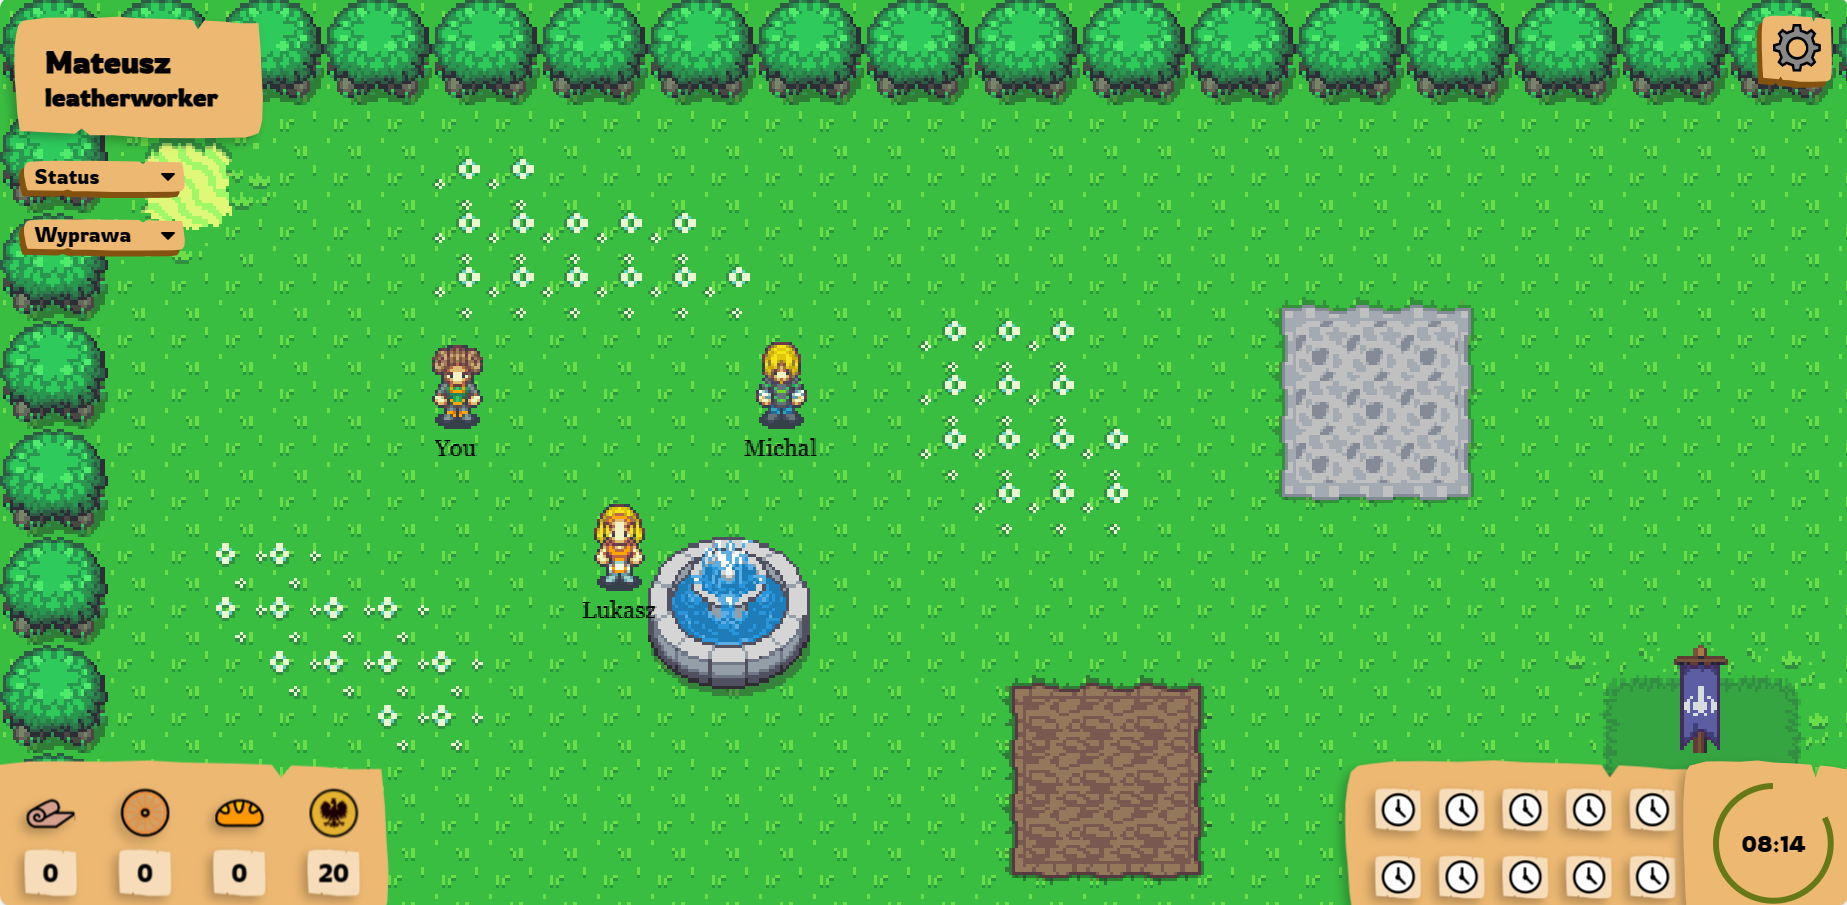
\includegraphics[width=1\linewidth]{resources/game_1.png}
    \caption{Ekran powitalny ECSB}
    \label{fig:stateful}
\end{figure}

eCSB jest aplikacją webową opartą o mikroserwisy oraz komunikację z wykorzystaniem wiadomości. W minimalnym wariancie składa się z 6 bezstanowych modułów napisanych w języku Kotlin, podłączonych do bazy danych Postgres, bazy klucz-wartość Redis oraz brokera wiadomości RabbitMQ, a także aplikacji webowej, komunikującej się z modułami poprzez protokoły REST oraz WebSocket. Dostęp do wszystkich elementów architektury realizowany jest dzięki serwerowi HTTP nginx, który pełni rolę reverse-proxy (zapewniając przy tym certyfikaty SSL i ruch HTTPS) oraz API gateway (przekierowując żądania do odpowiednich mikroserwisów). Pełna architektura rozwiązania przedstawiona jest poniżej \ref{fig:schema}.

\begin{figure}[h!]
    \centering
    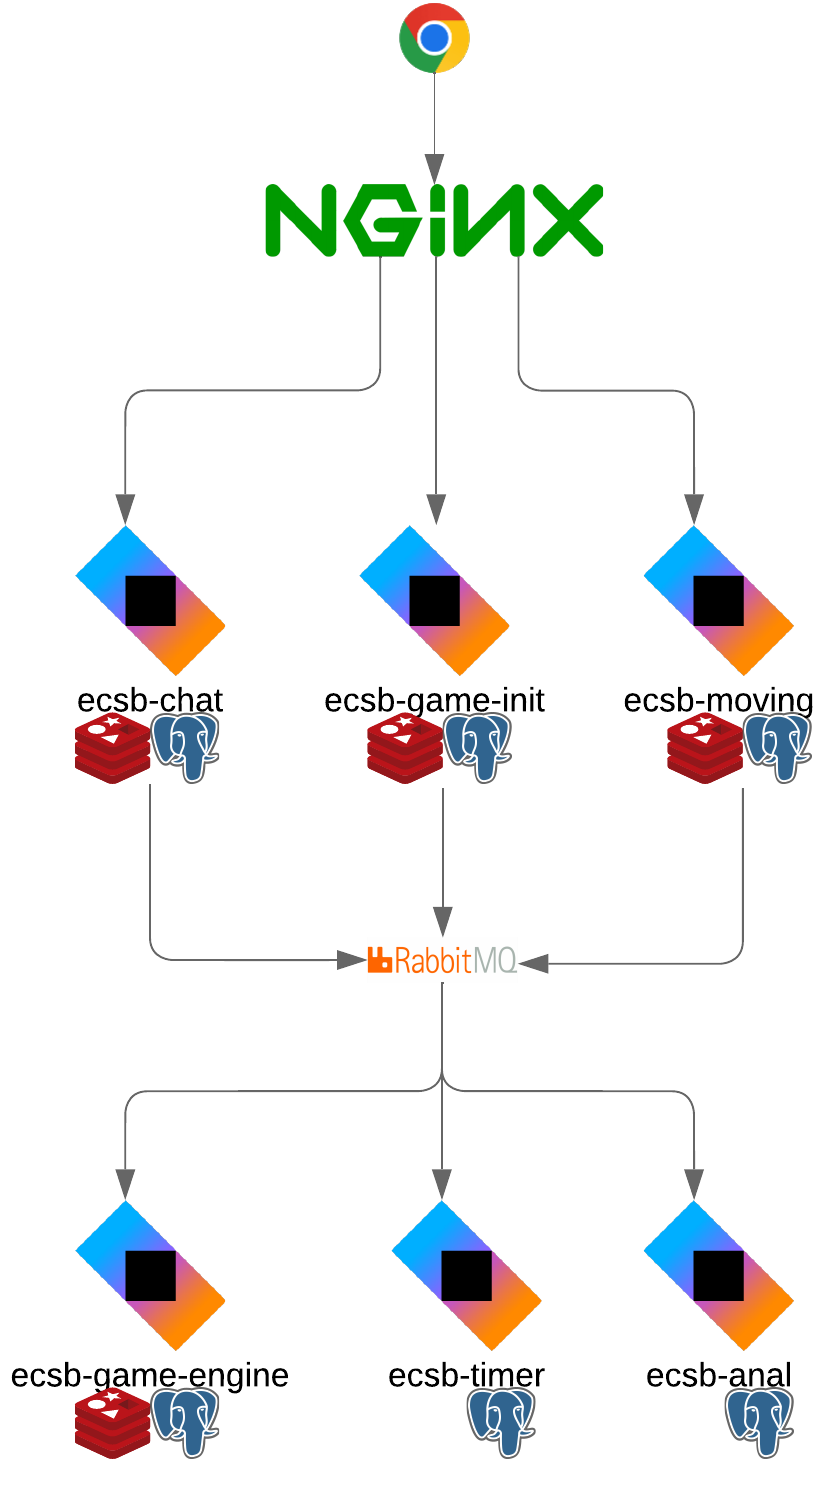
\includegraphics[width=0.8\linewidth]{resources/ecsb-schema.png}
    \caption{Architektura projektu eCSB}
    \label{fig:schema}
\end{figure}

\newpage
Warto dodać, że niektóre z modułów zostały zaprojektowane z myślą o skalowaniu systemu i rozkładaniu obciążenia. Są to moduły chat, moving oraz game-engine. Pozostałe 3 moduły odpowiadają za usługi stosunkowo rzadkie (tworzenie sesji gry) lub w pełni scentralizowane (zbieranie logów, odświeżanie czasu gry). 

\section{Przypadek użycia Operatora}

Naszym scenariuszem, poprzez który zademonstrujemy działanie Operatora dla aplikacji eCSB, będą następujące operacje:

\begin{enumerate}
    \item uruchomienie klastra Kubernetesowego z minimalnym wariantem eCSB (5 modułów - pomijamy moduł ecsb-anal, który służył jedynie do zbierania danych analitycznych)
    \item potrojenie skalowalnych modułów (moving, chat, game-engine), a następnie powrót do wariantu minimalnego
    \item przywrócenie centralnego modułu po awarii (timer lub game-init)
\end{enumerate}

%%%%%%%%%%%%%%%%%%%%%%%%%%%%%%%%%%%%%%%%%%%%%%%%%%%%%%%%%%%%%%%%%%%%%%%%%%%%%%%

\chapter{\ChapterTitleSolutionArchitecture}
\label{sec:architektura}

\begin{figure}[h!]
    \centering
    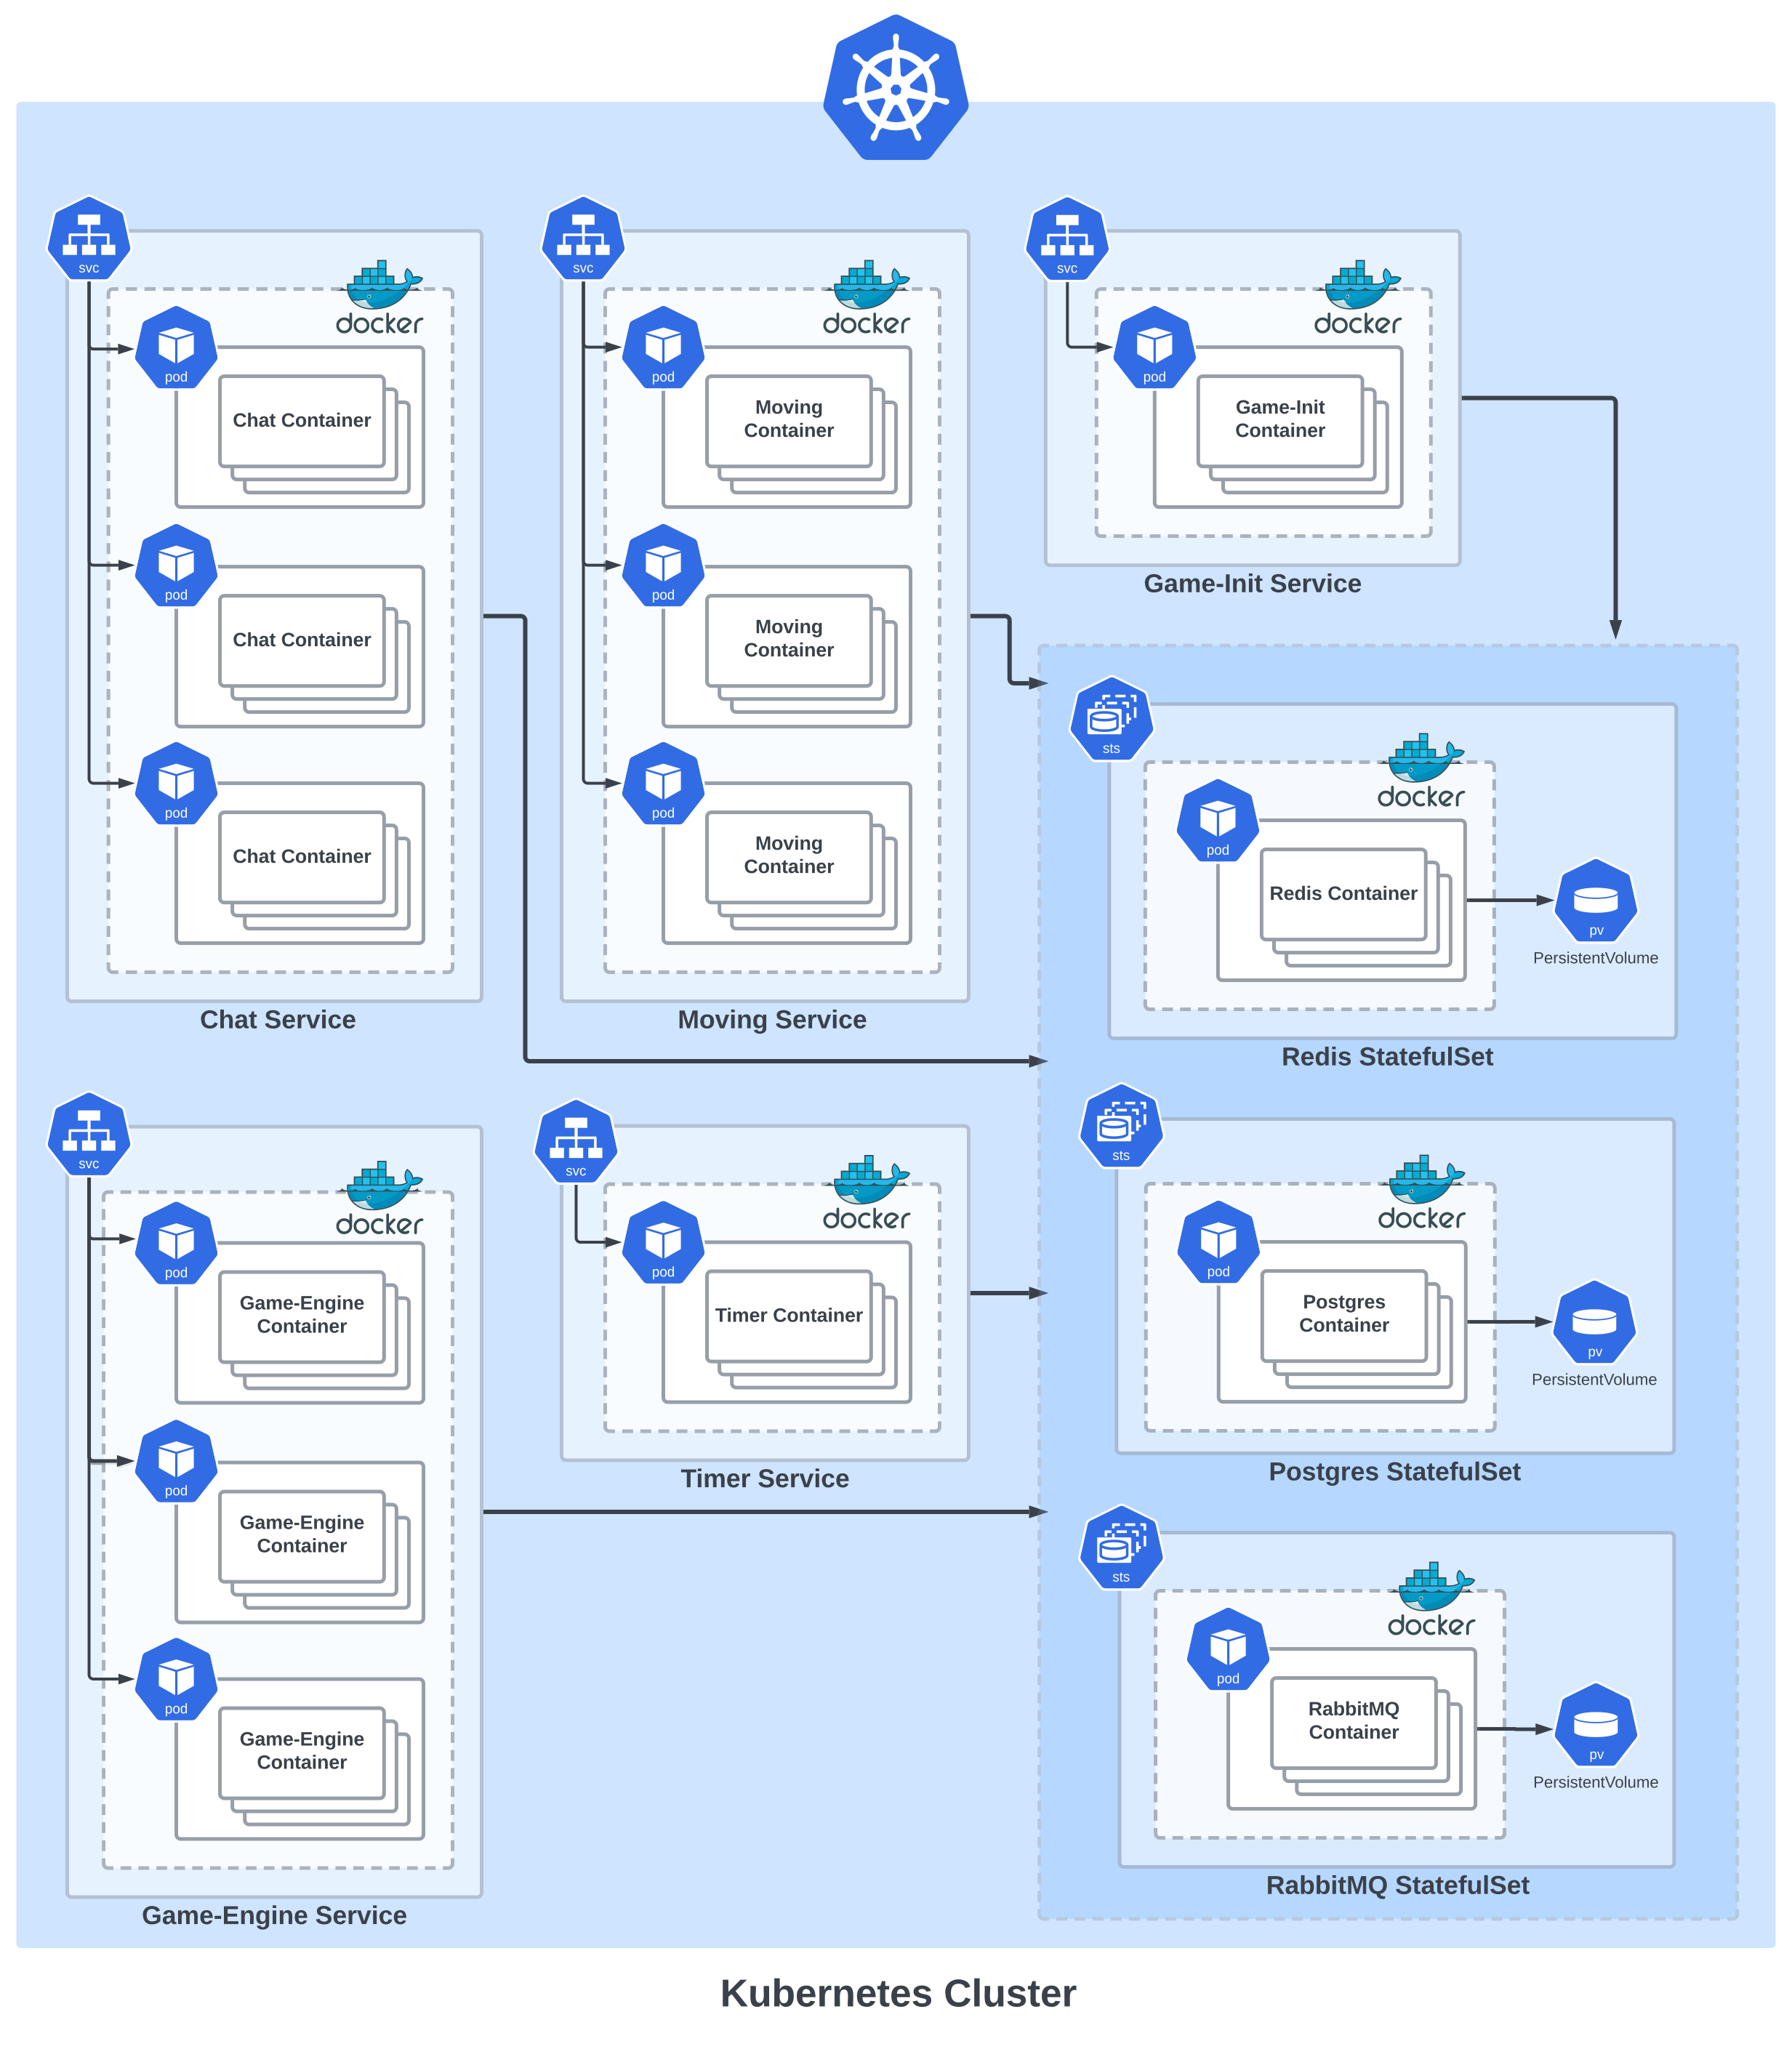
\includegraphics[width=0.9\linewidth]{resources/architecture_diagram.png}
    \caption{Diagram architektury rozwiązania z wykorzystaniem Kubernetesa}
    \label{fig:schema}
\end{figure}

%%%%%%%%%%%%%%%%%%%%%%%%%%%%%%%%%%%%%%%%%%%%%%%%%%%%%%%%%%%%%%%%%%%%%%%%%%%%%%%
\chapter{\ChapterTitleEnvConfig}
\label{sec:konfiguracja-srodowiska}

Jako punkt wyjścia konfiguracji naszego projektu wyznaczyliśmy zmodyfikowany plik docker-compose.yml, za pomocą którego uruchamiane było middleware dla aplikacji backendowych oraz aplikacja webowa. Rozszerzyliśmy go o backendowe mikroserwisy i dodaliśmy wstępną konfigurację dla PostgreSQL oraz RabbitMQ: 
\\
\begin{lstlisting}[caption=Przykład pliku Dockerfile dla mikroserwisu]
FROM gradle:7-jdk11 AS build
COPY .. /home/gradle/ecsb-backend
WORKDIR /home/gradle/ecsb-backend
RUN gradle :ecsb-game-engine:buildFatJar --no-daemon

FROM openjdk:11
WORKDIR /home/gradle/ecsb-backend
RUN mkdir /app
COPY --from=build 
/home/gradle/ecsb-backend/ecsb-game-engine/build/libs/*.jar 
/app/ecsb-game-engine.jar
ENTRYPOINT ["java", "-jar", "/app/ecsb-game-engine.jar"]
\end{lstlisting}

\begin{lstlisting}[caption=Przykładowa definicja kontenera mikroserwisu w pliku docker-compose.yml]
game-engine:
    container_name: game-engine
    build:
      context: ecsb-backend
      dockerfile: ./ecsb-game-engine/Dockerfile
    depends_on:
      - postgres
      - redis
      - rabbitmq
      - chat
    restart: on-failure
\end{lstlisting}

Mając z grubsza zdefiniowane kontenery składające się na architekturę, następnym krokiem było opakowanie ich w Kubernetesowe serwisy oraz konfiguracja zmiennych środowiskowych.

%%%%%%%%%%%%%%%%%%%%%%%%%%%%%%%%%%%%%%%%%%%%%%%%%%%%%%%%%%%%%%%%%%%%%%%%%%%%%%%
\chapter{\ChapterTitleInstallMethod}
\label{sec:instalacja}


%%%%%%%%%%%%%%%%%%%%%%%%%%%%%%%%%%%%%%%%%%%%%%%%%%%%%%%%%%%%%%%%%%%%%%%%%%%%%%%
\chapter{\ChapterTitleSolutionSteps}
\label{sec:odtworzenie}

%%%%%%%%%%%%%%%%%%%%%%%%%%%%%%%%%%%%%%%%%%%%%%%%%%%%%%%%%%%%%%%%%%%%%%%%%%%%%%%
\chapter{\ChapterTitleDemoDeployment}
\label{sec:deployment}

%%%%%%%%%%%%%%%%%%%%%%%%%%%%%%%%%%%%%%%%%%%%%%%%%%%%%%%%%%%%%%%%%%%%%%%%%%%%%%%
\chapter{\ChapterTitleSummary}
\label{sec:podsumowanie}


%%%%%%%%%%%%%%%%%%%%%%%%%%%%%%%%%%%%%%%%%%%%%%%%%%%%%%%%%%%%%%%%%%%%%%%%%%%%%%%

\section{Rysunki, tabele}
\label{sec:rysunki-tabele}

\subsection{Rysunki}
\label{sec:rysunki}

Przykładowy odnośnik do rysunku~\ref{fig:ex1}.

\begin{figure}[!htbp]
  \centering
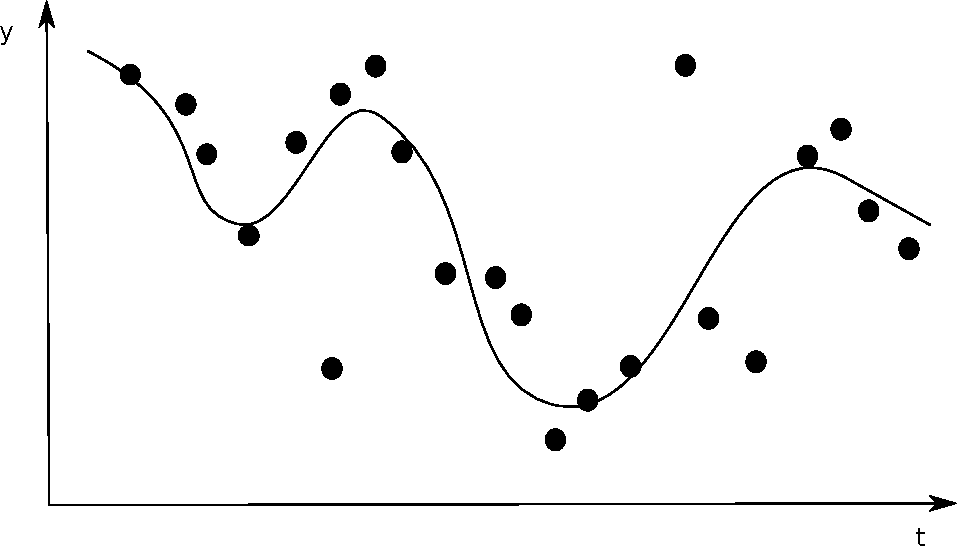
\includegraphics[width=.7\textwidth]{resources/example.pdf}
\caption[Przykładowy rysunek]{Przykładowy rysunek (źródło:
  \cite{author2021title})}
\label{fig:ex1}
\end{figure}
 
W przypadku rysunków można odwoływać się zarówno do poszczególnych części
składowych --- rysunek~\ref{fig:sub1} i rysunek~\ref{fig:sub2}) --- jak i do
całego rysunku~\ref{fig:ex2}.

\begin{figure}[!htbp]
\begin{center}
\subfigure[Tytuł 1]{%
\label{fig:sub1}
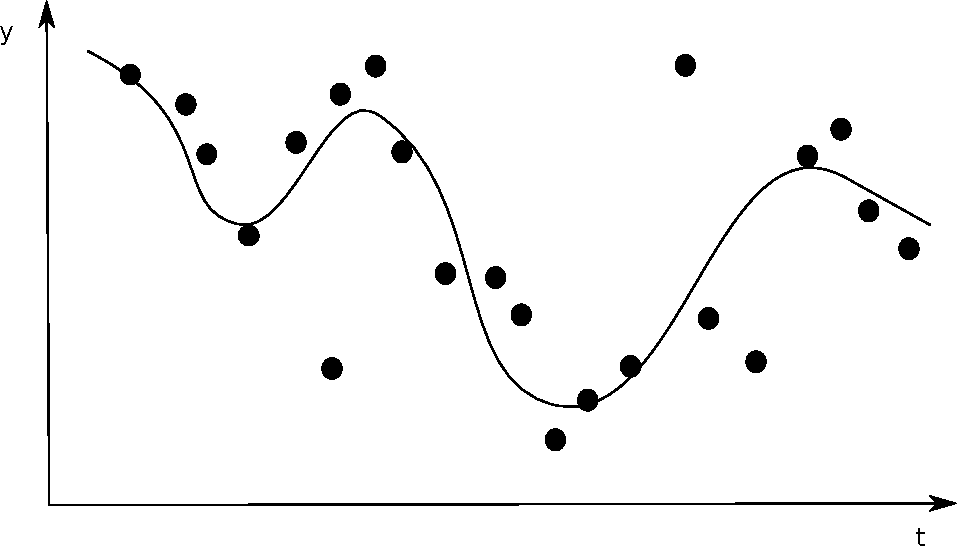
\includegraphics[width=0.48\textwidth]{resources/example.pdf}}%
\subfigure[Tytuł 2]{%
\label{fig:sub2}
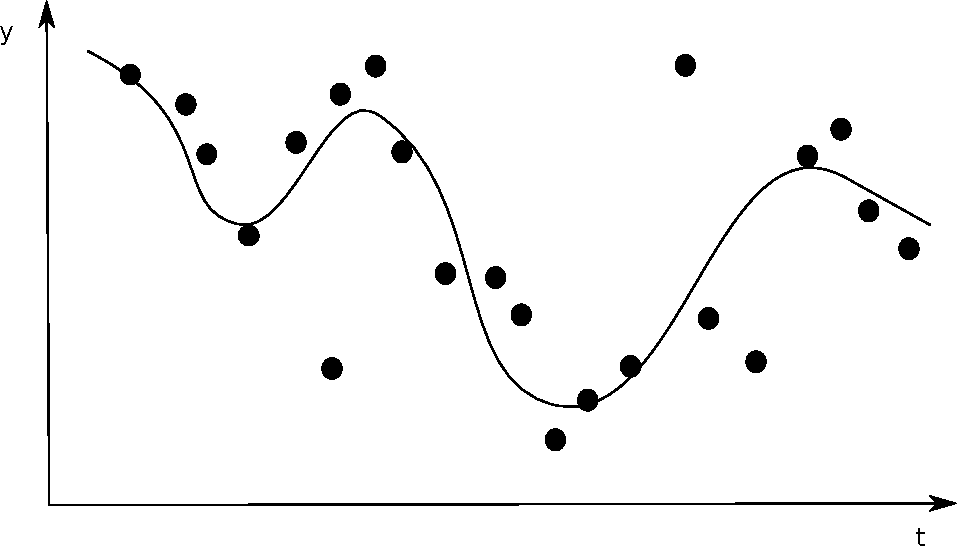
\includegraphics[width=0.48\textwidth]{resources/example.pdf}}
\end{center}
\caption[Kolejne przykładowe rysunki]{Kolejne przykładowe rysunki (źródło:
  \cite{author2021title})}
\label{fig:ex2}
\end{figure}

%%%%%%%%%%%%%%%%%%%%%%%%%%%%%%%%%%%%%%%%%%%%%%%%%%%%%%%%%%%%%%%%%%%%%%%%%%%%%%% 
\subsection{Tabele}
\label{sec:tabele}

Przykładowa tabela~\ref{tab:ex1}.

\begin{table}[!htbp]
\centering
\caption[Przykładowa tabela]{Przykładowa tabela}
\begin{tabularx}{\columnwidth}{@{}YYYYYYY@{}} \toprule
  & \multicolumn{2}{c}{\small\textbf{Best}} & \multicolumn{2}{c}{\small\textbf{Average}} & \multicolumn{2}{c}{\small\textbf{Worst}} \\ \cmidrule(lr){2-3} \cmidrule(lr){4-5} \cmidrule(lr){6-7}
  \textbf{No.} & \textbf{AB} & \textbf{CD} & \textbf{FE} & \textbf{GH} & \textbf{IJ} & \textbf{KL} \\ \midrule
  \textit{1.} & 10 & 89 & 58 & 244 & 6 & 70 \\  
  \textit{2.} & 15 & 87 & 57 & 147 & 4 & 82 \\
  \textit{3.} & 23 & 45 & 55 & 151 & 2 & 38 \\
  \textit{4.} & 34 & 90 & 55 & 246 & 1 & 82 \\
  \textit{5.} & 56 & 75 & 54 & 255 & 0 & 73 \\ \bottomrule
\end{tabularx}
\label{tab:ex1}
\end{table}

%%%%%%%%%%%%%%%%%%%%%%%%%%%%%%%%%%%%%%%%%%%%%%%%%%%%%%%%%%%%%%%%%%%%%%%%%%%%%%%
\section{Wzory matematyczne}
\label{sec:wzory}

% poniższy tekst należy usunąć z finalnej wersji pracy.

Przykład wzoru z odnośnikiem do literatury~\cite{author2021title}:

\begin{equation}
\Omega = \sum_{i=1}^n \gamma_i
\label{eq:sum}
\end{equation}

Przykładowy odnośnik do wzoru~\eqref{eq:sum}.

Przykładowy wzór w tekście $\lambda = \sum_{i=1}^n \delta_i$, bez numeracji.

%%%%%%%%%%%%%%%%%%%%%%%%%%%%%%%%%%%%%%%%%%%%%%%%%%%%%%%%%%%%%%%%%%%%%%%%%%%%%%%
\section{Cytowania}
\label{sec:cytowania}

Przykład cytowania literatury~\cite{wilson2009prediction-interday}. Kolejny przykład
cytowania kilku pozycji bibliograficznych~\cite{allen1999using-genetic, zitzler1999evolutionary-algorithms, pictet1995genetic-algorithms, wilhelmstotter2021jenetics, chmaj2015DistributedProcessingApplications}.
%%%%%%%%%%%%%%%%%%%%%%%%%%%%%%%%%%%%%%%%%%%%%%%%%%%%%%%%%%%%%%%%%%%%%%%%%%%%%%%
\section{Listy}
\label{sec:listy}

Lista z elementami:
\begin{itemize}
\item pierwszym,
\item drugim,
\item trzecim.
\end{itemize}

Lista numerowana z dłuższymi opisami:
\begin{enumerate}
\item Pierwszy element listy.
\item Drugi element listy.
\item Trzeci element listy.
\end{enumerate}
%%%%%%%%%%%%%%%%%%%%%%%%%%%%%%%%%%%%%%%%%%%%%%%%%%%%%%%%%%%%%%%%%%%%%%%%%%%%%%%
\section{Algorytmy}
\label{sec:algorytmy}

Algorytm~\ref{alg:pseudo-code} przedstawia przykładowy algorytm zaprezentowany w~\cite{fiorio2017algorithm2e}. 

\begin{algorithm}[!htbp]
\SetKwData{Left}{left}\SetKwData{This}{this}\SetKwData{Up}{up}
\SetKwFunction{Union}{Union}\SetKwFunction{FindCompress}{FindCompress}
\SetKwInOut{Input}{input}\SetKwInOut{Output}{output}
\Input{A bitmap $Im$ of size $w\times l$}
\Output{A partition of the bitmap}
\BlankLine
\emph{special treatment of the first line}\;
\For{$i\leftarrow 2$ \KwTo $l$}{
\emph{special treatment of the first element of line $i$}\;
\For{$j\leftarrow 2$ \KwTo $w$}{\label{forins}
\Left$\leftarrow$ \FindCompress{$Im[i,j-1]$}\;
\Up$\leftarrow$ \FindCompress{$Im[i-1,]$}\;
\This$\leftarrow$ \FindCompress{$Im[i,j]$}\;
\If(\tcp*[h]{O(\Left,\This)==1}){\Left compatible with \This}{\label{lt}
\lIf{\Left $<$ \This}{\Union{\Left,\This}}
\lElse{\Union{\This,\Left}}
}
\If(\tcp*[f]{O(\Up,\This)==1}){\Up compatible with \This}{\label{ut}
\lIf{\Up $<$ \This}{\Union{\Up,\This}}
\tcp{\This is put under \Up to keep tree as flat as possible}\label{cmt}
\lElse{\Union{\This,\Up}}\tcp*[h]{\This linked to \Up}\label{lelse}
}
}
\lForEach{element $e$ of the line $i$}{\FindCompress{p}}
}
  \caption[Przykładowy algorytm]{Przykładowy algorytm (źródło: \cite{fiorio2017algorithm2e}).}
  \label{alg:pseudo-code}
\end{algorithm}

%%%%%%%%%%%%%%%%%%%%%%%%%%%%%%%%%%%%%%%%%%%%%%%%%%%%%%%%%%%%%%%%%%%%%%%%%%%%%%% 
\section{Fragmenty kodu źródłowego}
\label{sec:listingi}
Listing~\ref{lst:maximum} przedstawia przykładowy fragment kodu źródłowego.

\begin{lstlisting}[language=Python,float=!htbp,caption={[Przykładowy fragment kodu]Przykładowy fragment kodu (źródło:
  \cite{author2021title})},label=lst:maximum]
# The maximum of two numbers

def maximum(x, y):

    if x >= y:
        return x
    else:
        return y

x = 2
y = 6
print(maximum(x, y),"is the largest of the numbers ", x, " and ", y)

\end{lstlisting}

%%%%%%%%%%%%%%%%%%%%%%%%%%%%%%%%%%%%%%%%%%%%%%%%%%%%%%%%%%%%%%%%%%%%%%%%%%%%%%%
\printbibliography

%%%%%%%%%%%%%%%%%%%%%%%%%%%%%%%%%%%%%%%%%%%%%%%%%%%%%%%%%%%%%%%%%%%%%%%%%%%%%%%
\listoffigures
\listoftables
\listofalgorithmes
\lstlistoflistings

\end{document}
